\documentclass[11pt,]{article}
\usepackage[left=1in,top=1in,right=1in,bottom=1in]{geometry}
\newcommand*{\authorfont}{\fontfamily{phv}\selectfont}

\usepackage[]{mathpazo}


  \usepackage[T1]{fontenc}
  \usepackage[utf8]{inputenc}

\usepackage{abstract}
\renewcommand{\abstractname}{}    % clear the title
\renewcommand{\absnamepos}{empty} % originally center

\renewenvironment{abstract}
 {{%
    \setlength{\leftmargin}{0mm}
    \setlength{\rightmargin}{\leftmargin}%
  }%
  \relax}
 {\endlist}

\makeatletter
\def\@maketitle{%
  \newpage
%  \null
%  \vskip 2em%
%  \begin{center}%
  \let \footnote \thanks
    {\fontsize{18}{20}\selectfont\raggedright  \setlength{\parindent}{0pt} \@title \par}%
}
%\fi
\makeatother




\setcounter{secnumdepth}{0}


\usepackage{graphicx,grffile}
\makeatletter
\def\maxwidth{\ifdim\Gin@nat@width>\linewidth\linewidth\else\Gin@nat@width\fi}
\def\maxheight{\ifdim\Gin@nat@height>\textheight\textheight\else\Gin@nat@height\fi}
\makeatother
% Scale images if necessary, so that they will not overflow the page
% margins by default, and it is still possible to overwrite the defaults
% using explicit options in \includegraphics[width, height, ...]{}
\setkeys{Gin}{width=\maxwidth,height=\maxheight,keepaspectratio}

\title{Lab 1: Cemetery demography \& life history strategies \thanks{\textbf{Current version}: January , 2019}  }



\author{\Large BIO 3103\vspace{0.05in} \newline\normalsize\emph{Baylor University}  }


\date{}

\usepackage{titlesec}

\titleformat*{\section}{\Large\bfseries}
\titleformat*{\subsection}{\normalsize\itshape}
\titleformat*{\subsubsection}{\normalsize\itshape}
\titleformat*{\paragraph}{\normalsize\itshape}
\titleformat*{\subparagraph}{\normalsize\itshape}





\newtheorem{hypothesis}{Hypothesis}
\usepackage{setspace}

\makeatletter
\@ifpackageloaded{hyperref}{}{%
\ifxetex
  \PassOptionsToPackage{hyphens}{url}\usepackage[setpagesize=false, % page size defined by xetex
              unicode=false, % unicode breaks when used with xetex
              xetex]{hyperref}
\else
  \PassOptionsToPackage{hyphens}{url}\usepackage[unicode=true]{hyperref}
\fi
}

\@ifpackageloaded{color}{
    \PassOptionsToPackage{usenames,dvipsnames}{color}
}{%
    \usepackage[usenames,dvipsnames]{color}
}
\makeatother
\hypersetup{breaklinks=true,
            bookmarks=true,
            pdfauthor={BIO 3103 (Baylor University)},
             pdfkeywords = {},  
            pdftitle={Lab 1: Cemetery demography \& life history strategies},
            colorlinks=true,
            citecolor=blue,
            urlcolor=blue,
            linkcolor=magenta,
            pdfborder={0 0 0}}
\urlstyle{same}  % don't use monospace font for urls

% set default figure placement to htbp
\makeatletter
\def\fps@figure{htbp}
\setlength{\intextsep}{25pt}  % sets space after text/before float figure
\makeatother



% add tightlist ----------
\providecommand{\tightlist}{%
\setlength{\itemsep}{0pt}\setlength{\parskip}{0pt}}

\begin{document}
	
% \pagenumbering{arabic}% resets `page` counter to 1 
%


% \maketitle

{% \usefont{T1}{pnc}{m}{n}
\setlength{\parindent}{0pt}
\thispagestyle{plain}
{\fontsize{18}{20}\selectfont\raggedright 
\maketitle  % title \par  

}

{
   \vskip 13.5pt\relax \normalsize\fontsize{11}{12} 
\textbf{\authorfont BIO 3103} \hskip 15pt \emph{\small Baylor University}   

}

}




\noindent  \hypertarget{background-information}{%
\section{Background information}\label{background-information}}

Organisms have evolved different \textbf{life history strategies} which
differ in their methods of reproduction, number and size of offspring,
timing of growth, means of resource acquisition, and prey avoidance.
Life history strategies are evolved traits that maximize reproductive
success in some way. However, resources are finite and for every benefit
a trait conveys to the organism it is normally associated with a
trade-off in the fitness of another trait. While these factors and how
they interact can be highly complex, \textbf{survivorship} offers a
simple means to quantify how a particular population ensures their
reproductive success.

For example, humans devote an enormous amount of energy and resources to
offspring care, which results in low mortality rates among their young.
On the other hand, most insects produce a massive number of offspring
that have extremely high rates of mortality, but due to the abundant
offspring some still survive to reproduce. Plotting the number of
surviving organisms against age yields what is called a
\textbf{survivorship curve} (Fig. 1), which is a visual way to assess
how various organisms differ in their life history strategies.
Scientists can use these plots to examine differences in organisms, or
assess changes within subsets of a population.

\begin{figure}
\centering
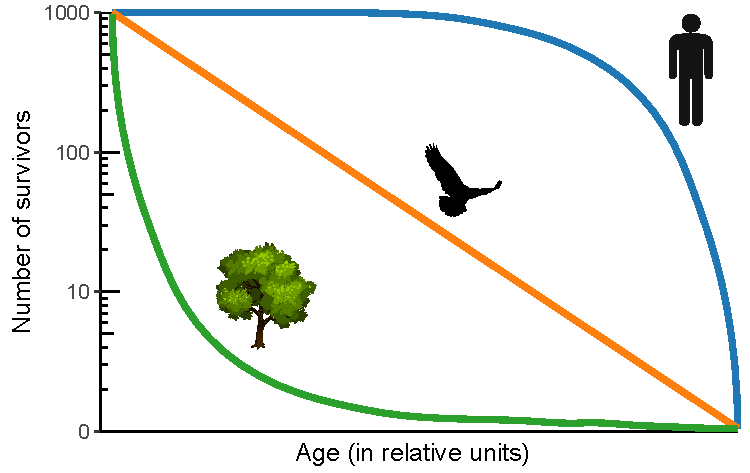
\includegraphics{../_chapter_materials/base_plot.pdf}
\caption{Idealized examples of Types I, II, and III survivorship curves
overlaid with example organisms. Type I survivorship is characterized by
high probability of survival early in life, followed by a rapid decline
as individuals reach older age. Type II survivorship displays roughly
constant mortality throughout the lifespan of the organism, and Type III
exhibits high mortality among young offspring.}
\end{figure}

\hypertarget{objectives}{%
\section{Objectives}\label{objectives}}

For this analysis you will use what you know about humans (\emph{Homo
sapiens}) and a common bird of prey (\emph{Aquila chrysaetos}, the
Golden Eagle) to form hypotheses about their life history strategies.
You will use demographic data collected from a local cemetery, as well
as data generated by the U.S. Fish \& Wildlife Service to address your
hypotheses about these two populations. We also have some ancillary data
collected from each individual (\textbf{ancillary data} is data
collected other than our primary variable of interest), which we can use
to divide the populations into two groups to see how different forces
influence survivorship \emph{within} a population.

\begin{figure}
\centering
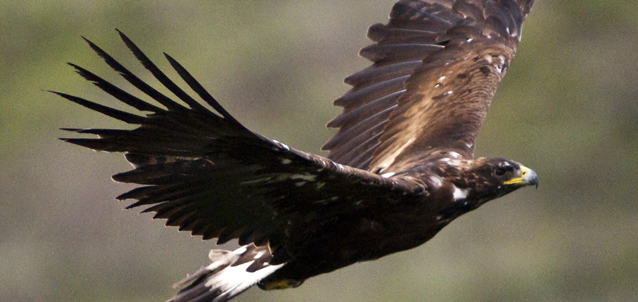
\includegraphics{../_chapter_materials/golden_eagle.jpg}
\caption{Migratory Golden eagle in Denali National Park and Preserve.
Mating pairs return each year to northern nesting territory in the
spring, and most new fledglings leave the nest by mid-August. During
winter their range extends from southern Canada to south of the Rocky
Mountains.}
\end{figure}

\begin{itemize}
\item
  We can use birth and death years on gravestones, as well as names (to
  infer gender) to collect simple but useful information about the local
  human population. You helped collect this data, and should be able to
  tell the reader how and why you did this.
\item
  Additionally, survey data collected by state and federal agencies
  provide valuable information about golden eagles. Golden eagles are
  federally protected in the United States, and Fish \& Wildlife
  collects detailed information from tagged individuals (Fig. 2). Every
  tagged individual is monitored till death, and afterwards detailed
  information about mortality is recorded along with the eagle's age. In
  this dataset, eagles are broadly divided into a group that died of
  natural causes and those that died from anthropogenic sources
  (power-lines, vehicle/boat hits, illegal hunting, etc.). This data was
  pulled from a report published by the U.S. Fish \& Wildlife Service
  (Milsap et al.~2016).
\end{itemize}

\pagebreak

We will use this data to test hypotheses addressing the following
questions:

\begin{enumerate}
\def\labelenumi{\arabic{enumi}.}
\tightlist
\item
  Does gender affect survivorship in human populations?

  \begin{itemize}
  \tightlist
  \item
    And if so, how?
  \end{itemize}
\item
  Does human impact affect survivorship in eagle populations?

  \begin{itemize}
  \tightlist
  \item
    And if so, how?
  \end{itemize}
\item
  Do humans and eagles display different life history strategies?
\end{enumerate}

Please form testable null hypotheses to address these questions. If you
want, you may also substitute question 1 for another within-population
comparison for humans. To evaluate your hypotheses, you will\ldots{}

\begin{enumerate}
\def\labelenumi{\arabic{enumi}.}
\tightlist
\item
  Questions 1 and 2: statistically address differences in survivorship
  between groups using a \textbf{t-test}, and display the data using a
  \textbf{bar-graph}
\item
  Question 3: \textbf{compute} and \textbf{display survivorship} (no
  statistical test needed for this part, assessing differences in those
  curves statistically is beyond the scope of this lab).
\end{enumerate}

\pagebreak

\hypertarget{lab-report-specifics}{%
\section{Lab report specifics}\label{lab-report-specifics}}

Below are some specific guidelines for this lab report, but you should
also utilize the general grading rubric in the Syllabus!

\begin{itemize}
\item
  \textbf{Participation} (1 pts)
\item
  \textbf{Introduction} (2 pts)

  \begin{itemize}
  \tightlist
  \item
    General information about population ecology / life history
    strategies
  \item
    How are survivorship curves used in population ecology?
  \item
    Build up rationale to lead into your objectives/hypotheses
    statements
  \end{itemize}
\item
  \textbf{Methods} (2 pts)

  \begin{itemize}
  \tightlist
  \item
    Explanation of data collection and analysis
  \end{itemize}
\item
  \textbf{Results} (5 pts)

  \begin{itemize}
  \tightlist
  \item
    Text section (overview of results, summary statistics, etc.)
  \item
    Bar-plots and associated t-tests for Q1 and Q2
  \item
    Survivorship curve for Q3
  \end{itemize}
\item
  \textbf{Discussion} (2 pts)

  \begin{itemize}
  \tightlist
  \item
    Clearly address your null hypotheses
  \item
    What are some plausible explanations for differences (or lack
    thereof) between groups?
  \item
    What are some plausible explanations for differences between humans
    and golden eagles?
  \item
    Place your results in an evolutionary context.
  \end{itemize}
\end{itemize}

\medskip

\hypertarget{literature-cited}{%
\section{Literature cited}\label{literature-cited}}

Ecologists frequently use publicly available data in their analyses.
While you do not need to cite the data-source, you do need to tell the
reader in your \textbf{Methods} section who generated the data, as well
as what parts of the dataset you used.

\medskip

Milsap, B. A., Bjerre, E. R., Otto, M. C., Zimmerman, G. S., \& Zimpfer,
N. L. (2016). Bald and Golden Eagles: Population demographics and
estimation of sustainable take in the United States, 2016 update
(p.~115). Division of Migratory Bird Management, Washington D.C., USA:
U.S. Fish and Wildlife Service.




\newpage
\singlespacing 
\end{document}
